\chapter{Standar Git}
Sebelum melakukan langkah \textit{pull request} alangkah baik anda mempelajari materi \textit{Git} di \textbf{\textit{https://github.com/BukuInformatika/git}} (buka git.pdf).

\section{Standar Git}
Langkah-langkah \textit{pull request} menggunakan \textit{GIT BASH} :
\begin{enumerate}
\item git fetch upstream seperti pada gambar ~\ref{fig:p1}
		\begin{figure}[H]
		\centering
		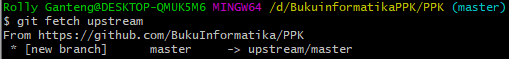
\includegraphics[width=1\textwidth]{figures/pullrequest/p1.PNG}
		\caption{Ini adalah perintah \textit{git fetch upstream}}
		\label{fig:p1}
		\end{figure}
\item git pull upstream master seperti pada gambar \ref{fig:p2}
		\begin{figure}[H]
		\centering
		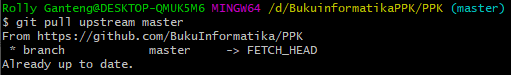
\includegraphics[width=1\textwidth]{figures/pullrequest/p2.PNG}
		\caption{Ini adalah perintah \textit{git pull upstream master}}
		\label{fig:p2}
		\end{figure}
\item edit file yang akan di pull request seperti pada gambar \ref{fig:p3}
		\begin{figure}[H]
		\centering
		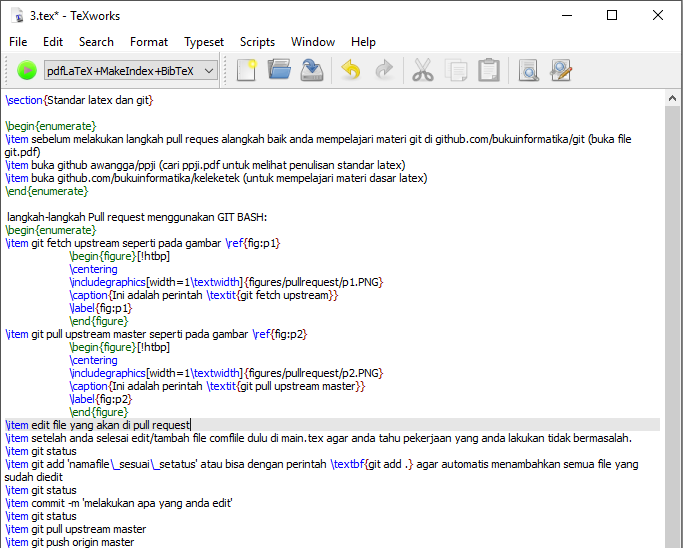
\includegraphics[width=1\textwidth]{figures/pullrequest/p3.PNG}
		\caption{Ini adalah halaman kerja yang siap untuk diedit}
		\label{fig:p3}
		\end{figure}
\item setelah anda selesai edit/tambah file comflile dulu di main.tex agar anda tahu pekerjaan yang anda lakukan tidak bermasalah. dengan memulai compile seperti pada gambar \ref{fig:p4}
		\begin{figure}[H]
		\centering
		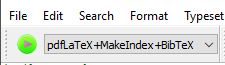
\includegraphics[width=1\textwidth]{figures/pullrequest/p4.PNG}
		\caption{Ini adalah langkah meng-compile}
		\label{fig:p4}
		\end{figure}
\item git status maka kita akan mengetahui apa saja yang belum ditambahkan seperti pada gambar \ref{fig:p5}
		\begin{figure}[H]
		\centering
		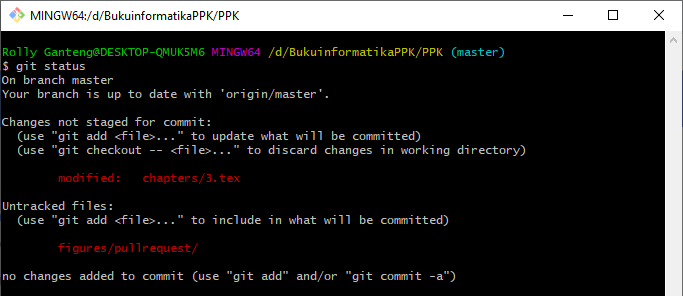
\includegraphics[width=1\textwidth]{figures/pullrequest/p5.PNG}
		\caption{Ini adalah perintah \textit{git status}}
		\label{fig:p5}
		\end{figure}
\item git add 'namafile\_sesuai\_setatus' atau bisa dengan perintah \textbf{git add .} agar automatis menambahkan semua file yang sudah diedit seperti pada gambar \ref{fig:p6}
		\begin{figure}[H]
		\centering
		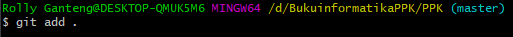
\includegraphics[width=1\textwidth]{figures/pullrequest/p6.PNG}
		\caption{Ini adalah perintah \textit{git add}}
		\label{fig:p6}
		\end{figure}
\item git status seperti pada gambar \ref{fig:p7}
		\begin{figure}[H]
		\centering
		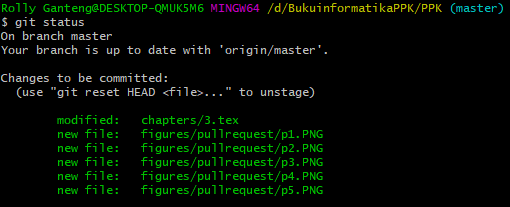
\includegraphics[width=1\textwidth]{figures/pullrequest/p7.PNG}
		\caption{Ini adalah perintah \textit{git status}}
		\label{fig:p7}
		\end{figure}
\item commit -m 'melakukan apa yang anda edit' seperti pada gambar \ref{fig:p8}
		\begin{figure}[H]
		\centering
		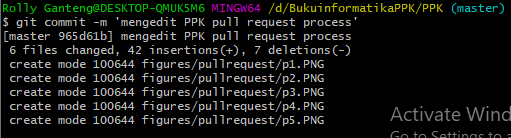
\includegraphics[width=1\textwidth]{figures/pullrequest/p8.PNG}
		\caption{Ini adalah perintah \textit{git commit}}
		\label{fig:p8}
		\end{figure}
\item git pull upstream master
		\begin{figure}[H]
		\centering
		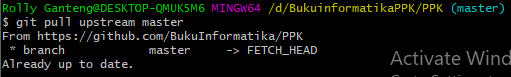
\includegraphics[width=1\textwidth]{figures/pullrequest/p9.PNG}
		\caption{Ini adalah perintah \textit{git pull upstream master}}
		\label{fig:p9}
		\end{figure}
\item git push origin master seperti pada gambar \ref{fig:p10}
		\begin{figure}[H]
		\centering
		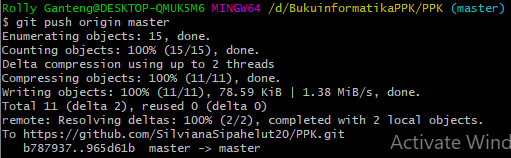
\includegraphics[width=1\textwidth]{figures/pullrequest/p10.PNG}
		\caption{Ini adalah perintah \textit{git push origin master}}
		\label{fig:p10}
		\end{figure}
\end{enumerate}

Buka repositori anda untuk new pull request:
\begin{enumerate}
\item Klik New Pull request pada gambar yang diberi tanda kotak warna merak \ref{labelgambar1}
		\begin{figure}[H]
		\centering
		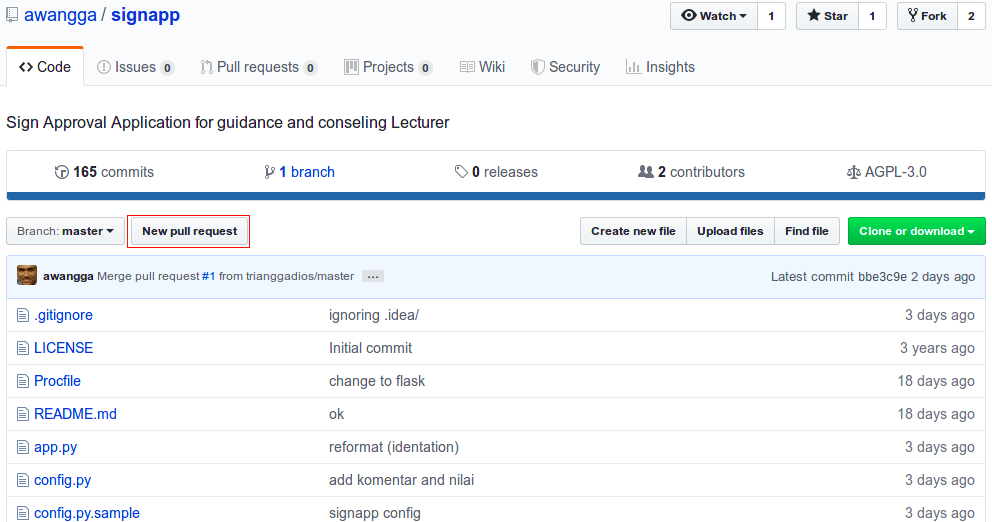
\includegraphics[width=1\textwidth]{figures/1.png}
		\caption{Gambar klik pull request}
		\label{labelgambar1}
		\end{figure}
\item Klik tombol hijau seperti pada gambar lihat tanda yang diberi kotak warna merah \ref{labelgambar2} 
		\begin{figure}[H]
		\centering
		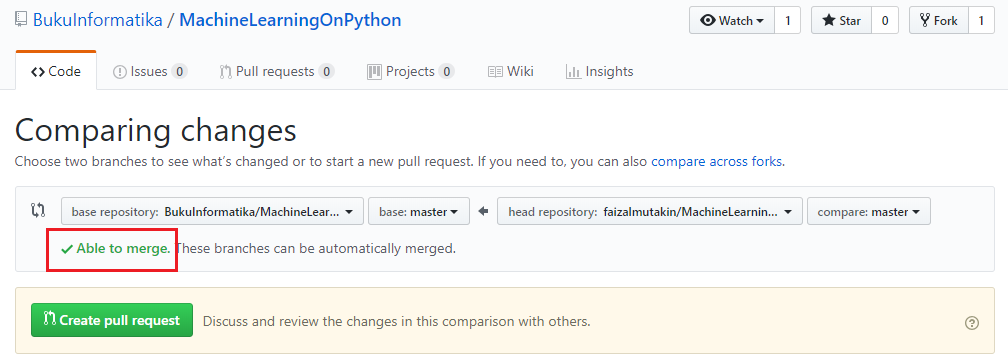
\includegraphics[width=1\textwidth]{figures/2.PNG}
		\caption{Gambar new pull request}
		\label{labelgambar2}
		\end{figure}	 
\end{enumerate}